\chapter{Perancangan}
\label{chap:perancangan}
Bab ini membahas perancangan untuk seluruh implementasi \textit{SharIF Judge} pada \textit{CodeIgniter 4}.

\section{Instalasi \textit{CodeIgniter 4}}
\textit{CodeIgniter 4} akan dilakukan instalasi menggunakan \textit{composer}. \textit{Composer} merupakan sebuah \textit{dependency manager} untuk PHP yang memungkinkan pengguna untuk melakukan instalasi seluruh kebutuhan untuk menjalankan program berbasis PHP. Instalasi akan dilakukan menggunakan kode sebagai berikut:

\section{Perubahan Struktur Aplikasi}
\label{sec:perubahanStruktur}
Struktur aplikasi \textit{SharIF Judge} akan dipindahkan seperti pemetaan pada gambar \ref{fig:dirMappingBab4}.

\begin{figure}[H]
	\centering  
	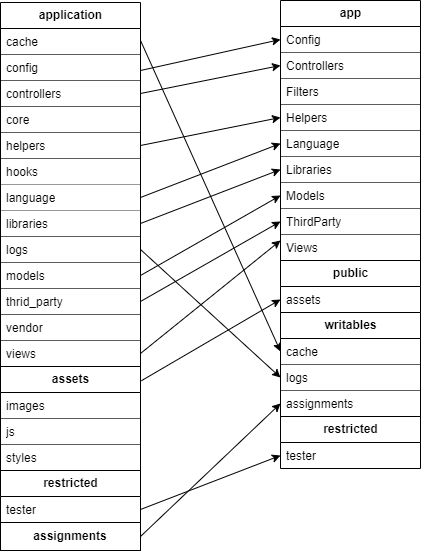
\includegraphics[scale=0.5]{dirMapping}  
	\caption[\textit{Pemindahan struktur aplikasi menuju \textit{CodeIgniter 4}}]{\textit{Pemindahan struktur aplikasi menuju \textit{CodeIgniter 4}}} 
	\label{fig:dirMappingBab4} 
\end{figure} 

Struktur aplikasi pada \textit{CodeIgniter 4} akan berisikan sebagai berikut :
\subsection{App}
\begin{itemize}
	\item \texttt{app/Config}\\ berisikan data-data pada \texttt{application/Config}. Terdapat juga penambahan \textit{file} \texttt{Secrets.php} dan juga pemindahan token menuju \texttt{app/Config/Security.php}.  
	\item \texttt{}\\ 
\end{itemize}
\section{Rancangan Perubahan Kode pada CodeIgniter 3 Menjadi CodeIgniter 4}
\label{sec:rancanganPerubahanKode}
Pada \textit{CodeIgniter 4} terdapat perubahan dan penghilangan fungsi-fungsi sehingga terdapat perubahan dan penggantian fungsi.
\subsection{Config}
\textit{File config} pada \textit{CodeIgniter 3} akan dipindahkan sesuai dengan pemetaan pada gambar .
\subsection{\textit{Model, View} dan \textit{Controller}}.
\subsubsection{\textit{Model}}
\textit{Model} akan dipindahkan sesuai dengan direktori \ref{sec:perubahanStruktur} dan diubah sesuai dengan dokumentasi \textit{CodeIgniter 4}. Seluruh \textit{Model} akan diganti penamaannya dari yang sebelumnya menggunakan \textit{snakecase} menjadi \textit{camelcase}.

\subsubsection{\textit{View}}
\textit{View} akan diubah menggunakan \textit{extension} \texttt{.php} sesuai pada dokumentasi \textit{CodeIgniter 4}. Seluruh \textit{file view} akan diubah menjadi \textit{extension} \texttt{.php} dari yang sebelumnya menggunakan \texttt{.twig}. Seluruh \textit{delimiters} juga akan diubah menggunakan fungsi pada \textit{CodeIgniter 4}. Perubahan \textit{view} dapat dilihat pada kode \ref{kode:loginViewBab4}.

\begin{lstlisting}[caption=Perubahan \textit{view} pada \textit{Login.php}, label=kode:loginViewBab4]
<!-- {#
 # SharIF Judge
 # file: login.twig
 # author: Mohammad Javad Naderi <mjnaderi@gmail.com>
 #} -->
<!DOCTYPE html>
<html lang="en">
<?= $this->include('templates/simple_header')?>

<?= form_open() ?>
	<div class="box login">

		<div class="judge_logo">
			<a href="<?= site_url() ?>"><img src="<?= base_url('assets/images/banner.png') ?>"/></a>
		</div>

		<div class="login_form">
			<div class="login1">
				<p>
					<label for="form_username">Username</label><br/>
					<input id="form_username" type="text" name="username" required="required" pattern="[0-9a-z]{3,20}" title="The Username field must be between 3 and 20 characters in length, and contain only digits and lowercase letters" class="sharif_input" value="<?= set_value('username') ?>" autofocus="autofocus"/>
					<?= isset($this->errors['username'])?>
				</p>
				<p>
					<label for="form_password">Password</label><br/>
					<input id="form_password" type="password" name="password" required="required" pattern=".{6,200}" title="The Password field must be at least 6 characters in length" class="sharif_input"/>
					<?= isset($this->errors['password'])?>
				</p>
				<?php if ($error): ?>
					<div class="shj_error">Incorrect username or password.</div>
				<?php endif ?>
			</div>
			<div class="login2">
				<p style="margin:0;">
					<?php if ($registration_enabled): ?>
					<a href="<?= site_url('register') ?>">Register</a> |
					<?php endif ?>
					<a href="<?= site_url('login/lost') ?>">Reset Password</a>
					<input type="submit" value="Login" id="sharif_submit"/>
				</p>
			</div>
		</div>

	</div>q
<?= form_close() ?>
</body>
</html>
\end{lstlisting}

Selain terdapat perubahan \textit{extension} dan \textit{delimiters}, terdapat juga penambahan kode pada \textit{Controller} karena tidak mendukung pembentukan variabel pada \textit{View}. Kode \ref{} merupakan contoh penambahan kode pada \textit{Controller}.

\begin{lstlisting}[caption=Perubahan \textit{view} pada \textit{Login.php}, label=kode:loginViewBab4]

\end{lstlisting}

\subsubsection{\textit{Controller}}
\textit{Controller} terdapat perubahan pada bagian \texttt{\_\_construct()} dimana sekarang tidak dapat mengembalikan sesuatu. Oleh karena itu, akan dibentuk beberapa \textit{filters} untuk melakukan pengecekan terhadap fungsi yang sebelumnya terdapat pada \texttt{\_\_construct()}.